\chapter{Soft Materials Modelling: Artificial Neural Networks}

\section{Introduction} 

In the previous chapter, a mathematical model for the prediction of viscoelastic behaviour in soft materials was developed. The PL-SLS model was able to successfully model the nonlinear stress response of seven soft materials. Nevertheless, the model was not able to account for the velocity-dependency response of the soft materials. The latter is critical to predict the time-dependent properties of commonly used soft materials in soft robotic applications. Therefore, an alternative approach is investigated.

The field of machine learning provides with reliable data-driven modelling tools, such as artificial neural networks (ANN). ANN have been successful in extracting complex mechanical parameters of soft materials, and are now being used to model the stress-strain curve of many materials. Nonetheless, the literature on soft materials is very scarce. Also, to the best of the author knowledge, the modelling of the velocity-dependency of the stress response of soft materials has not been performed. The latter is addressed in this chapter.

In this work, the developed ANN is a feedforward neural network. The Bayesian Regularization algorithm is used during the training process. The selection of inputs and outputs to be included to the network was optimized by observing the generalization capabilities of each proposed combination. Moreover, the optimal number of neurons was also optimized to avoid a common phenomenon known as over-fitting. The optimal number of neurons varies from one soft material to the other, but in any case exceed 10 neurons.

Finally, the generalization error of the developed ANN is compared against the previously developed PL-SLS model. In general, the developed ANN outperforms the PL-SLS model in both achievable error and generalization capabilities. Hence, the ANN is considered to successfully account for the velocity-dependent stress response of the materials.Nonetheless, the PL-SLS performs better than the ANN model for one single material, the SR material. This is correlated with the fact that the SR material is very elastic, hence its stress response is not dependent on the strain rate. This could play a role in the performance of the ANN which has the strain rate as input, creating confusion to the network rather than contributing to the learning process.

\section{Artificial Neural Networks}

Artificial Neural Networks (ANNs) are computational systems inspired in the structure and functionality of the biological nervous system. Neurons, a specific type of cell, are the basic components in the brain. They form connections with a vast number of other neurons, allowing us to remember, think, and apply previous knowledge to our present actions. The basic functionality of a neuron is to receive information in its inputs from many sources, to combine it, to apply a nonlinear operation, and to output the end result. Moreover, neurons are capable of specializing for a specific task by amplifying or reducing the impact of their individual inputs. Neurons are also capable of reorganizing themselves in complex interconnected clusters in a three-dimensional space, called biological neural networks, in where the information flows from one group of neurons to the other.

Similarly, Artificial Neural Networks are composed of many basic components, known as artificial neurons, working in parallel. The clustering found in biological neural networks, can be replicated in ANNs by creating layers, containing many neurons, which can be interconnected between each other in different ways. The simplest structure of an ANN is composed of three layers: and input layer, a hidden layer, and an output layer. As the name suggest, the input and output layers interface the ANN with the outside world. The main learning process happens in the hidden layer. The way in which the interconnections between these three layers are form, are mainly dependent on the application. The strength of each interconnection depends on a weighting factor, enabling the artificial neuron to amplify or reduce the contribution of a specific input. The fine tuning of this weights, performed in a process called training, allows ANNs to specialize in a particular task, i.e. allow them to learn. The latter highlights the capability of ANNs to simulate two key functionalities of the human brain, which are: acquiring knowledge from the environment through a learning process, and storing this knowledge in the form of inter-neuron connection strengths, i.e. synaptic weights. The capability of learning from experience, i.e. experimental data, make ANNs particularly useful when dealing with complex scientific and engineering problems where an adequate analytical description is not available, or is too complex  \cite{zhang2003artificial,trebar2007predicting}.

The most simple ANN configuration has at least one input layer, one hidden layer, and one output layer \Cref{fig:neruonANN}. Nonetheless, ANNs can have as many layers as desired, simulating the clustering phenomenon found in biological neural networks. These type of multi-layered ANNs can be categorized depending on how the information flows inside it. For example, a ANN in which the information flows in one direction, from the input layer up to the output layer, is called Feedforward Neural Network (FFNN). This type of ANN, illustrated in \Cref{fig:FFANN} is one of the most commonly used for function approximation, pattern recognition and classification \cite{zhang2003artificial}.

\begin{figure}[htb!]
	\centering
    \begin{subfigure}[b]{0.49\textwidth}
        \centering
        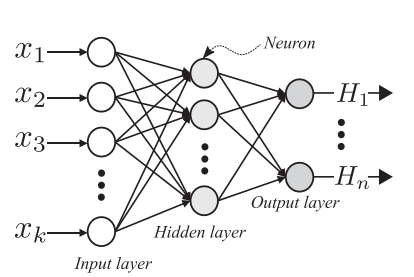
\includegraphics[width=\textwidth]{FeedForwardANN.PNG}
        \caption{}
        \label{fig:FFANN}
    \end{subfigure}
    \begin{subfigure}[b]{0.49\textwidth}
        \centering
        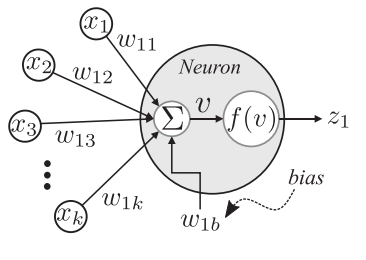
\includegraphics[width=\textwidth]{Neuron.PNG}
        \caption{}
        \label{fig:neuron}
    \end{subfigure}
    \caption{(a) Feedforward artificial neural network (b) Internal structure of an artificial neuron\cite{rodriguez2019application}}
    \label{fig:neruonANN}
\end{figure}

The variables illustrated in \Cref{fig:FFANN} are as follows. The inputs of the ANN are represented by the variable $\mathbf{x}$, in the form of:

\begin{equation}
    \mathbf{x} = [x_1, x_2, x_3, ... , x_k ]
    \label{c6_neuronin}
\end{equation}

\noindent where $k$ represents the total number of inputs. Similarly, the outputs of the ANN are represented by the variable $\mathbf{H}$ in the form of:

\begin{equation}
    \mathbf{H} = [H_1, H_2, H_3, ... , H_n ]
    \label{c6_networkout}
\end{equation}

\noindent where $n$ represents the total number of outputs. Furthermore, the output of the neuron illustrated in \Cref{fig:neuron}, combines the individual weighted values of the input vector $x$ with a bias value. Then, a nonlinear function is applied to the result of this sum. This is described as follows:

\begin{equation}
    z_1 = f \left( \sum_{i=1}^k(x_i w_{i,j}) + w_{1,bias} \right)
\label{c6_neuronout}
\end{equation}

\noindent where $w_{1,1}$ to $w_{1,k}$ represents the weights of one neuron which interacts with all the inputs. The first subscript the neuron these weights belong to, whereas the second subscript indicates the input to which a weight is related to. 

In order for the ANN to learn, they must be trained first. In FFNN the most common approach for training is called the Backpropagation Algorithm. The training process of ANN commonly involves dividing the available data into a training and a test subset. The former subset is used for training of the ANN, whereas, the latter is used for testing the prediction capabilities of the ANN aftet being trained. During training, the ANN is presented with known values of the output, called targets, which are related to a specific combination of inputs. In each training session the ANN will adapt slightly until its output is close to the target value. The backpropagation algorithm is based on minimizing the sum of square errors (SSE) between the target and predicted values, by modifying the weights and biased of the ANN \cite{zhang2003artificial}. This algorithm is so powerful in minimizing the error that it could cause the ANN to memorize the training dataset instead of generalizing it. This means that the ANN will not be able to provide accurate predictions when new data is presented to it. This issue is called over-fitting.

According to the literature, FFNN are capable of representing any functional relationship between a set of inputs and outputs, as long as the ANN has enough number of neurons in its hidden layers. However, having too many neurons increases risk of over-fitting. As previously mentioned, over-fitting will prevent the ANN to generalize well. Therefore, when designing an ANN is better to use the minimum amount of resources which are able to provide a good fit. There are two main methods for preventing over-fitting from happening, i.e. improving generalization, during the training process: early stopping and regularization. On the one hand, in the early stopping method, a third subset of data is involved, called the validation subset. In general terms, when the error during the validation process increases during certain number of consecutive training sessions, then over-fitting is detected and the training process is stopped. On the other hand, in a regularization method the performance function used during training, commonly the SEE of the ANN prediction, is modified. For example, in the Bayesian Regularization method, the performance function has an additional condition, which is to minimize the SSE of the weights and biases of the ANN. This prevents puts a check on the correction power from the backpropagation algorithm, which allows the weights and biased to be fine-tuned rather than have large variations. 

There are many variables involved in the process of designing and optimizing an ANN for a specific application. Therefore, the relevant works on implementation of ANN for the modelling of soft materials is presented as follows

\section{ANN for Modelling of Soft Materials }

Artificial Neural Networks have been implemented in a wide number of applications, such as: forecasting, control, power systems, robotics, signal processing, manufacturing, pattern recognition and optimization \cite{khan2019fabrication}. At the time of writing this document, the available literature about the implementation of ANNs for the modelling of the complex behaviour of soft materials, specifically elastomers, was scarce. However, recently there was a notorious increment in the published papers focusing on modelling soft materials using ANNs which highlights the relevance of this field of research.

One of the earliest works in this field is documented in \cite{zhang2002dynamic} by Zhang et al.. In here, a FFNN is developed to model the dynamic mechanical properties of short fibre reinforced materials. The trained ANN was able to provide prediction values for the storage modulus and damping of the material for temperature values not used during the training process. Many properties of the material are provided as input to the network. The developed ANN had 25 neurons in its single hidden layer with a tan-sigmoidal transfer function, whereas the output layer had a linear transfer function. The Bayesian Regularization algorithm was used for training. The prediction capabilities of the ANN were assessed using the percentage of correct predictions, in which a prediction with an R-squared value great than 0.9 is considered correct. The ANN was tested 50 times with a randomized test set each time. Moreover, the authors found a proportional relationship between the complexity of the parameters to model, and the amount of data required to train the ANN. 

The review paper of Zhang et al. about the implementation of ANNs in polymer composite applications, found that the available literature on the subject was scarce at that time \cite{zhang2003artificial}. Moreover, the documented applications ranged from modelling of the fatigue life of the material, to prediction of tribological and dynamic mechanical properties of composite materials \cite{zhang2002prediction,zhang2002dynamic}. This review paper provided very insightful evidence of the potential of ANNs for applications such as: design of new composite materials, optimization of the manufacturing process, and modelling the relationship between different manufacturing parameters. From the reviewed works, the authors were able to find a well defined sequence of actions which describes the process of implementing ANNs for the prediction of the mechanical properties of composite materials:

\begin{enumerate}
    \item \textbf{Data collection:} the first step in designing an ANN is to collect enough data from experimentation. On top of this, processing of the collected data, mainly to filter out noise, might be required.
    \item \textbf{ANN design and training:} the second step is to design the ANNs depending on the application at hand. This involves deciding on the best parameters to use, in terms of: number of neurons, number of hidden layers, training algorithm and neuron's activation function. Also, this step involves the training of the proposed ANN.
    \item \textbf{Test of the trained network:} this step is about assessing the prediction and generalization capabilities of the trained ANN. The former is commonly assessed by looking at the difference between predicted and experimental values, as a general rule, the lower the error, the better the prediction. The generalization of the network is assessed by statistical methods such as p-fold cross-validation and the coefficient of determination.
    \item \textbf{Use of the trained network:} the last step is to use the trained network to simulate new data or for prediction.
\end{enumerate}

The latter process highlights the large number of configurations available when tackling a modelling problem. Due to this, some works in the literature opt for a ``trial and error'' approach when investigating the potential of ANN for a specific application. Nonetheless, many works do perform optimizations in more than on of the ANN hyper-parameters. For example, motivated by the limitations of traditional viscoelastic models, the viscoelastic behaviour of polymer composites is assessed \cite{al2006prediction}. In here an ANN is developed to predict the stress relaxation characteristics of a polymer composite. The amount of data used in here is rather large, having 900 datasets covering different conditions of the stress relaxation process. The training algorithm used is the scaled conjugate gradient. In addition to this, the optimal brain surgeon algorithm is used to optimize the topology of the network. The latter algorithm assess the contribution of each neuron to the final results, by removing neurons one by one. This process is also known as pruning. The developed ANN had two hidden layers with 45 and 39 neurons, respectively; and was successful in modeling the stress relaxation characteristics of the material for ranges in which viscoelastic models were unsuccessful.

Initial works on this field of research were solely focus on one specific material. However, as the research matured, more materials were studied in a single work. This is the case for the work from Trebar et al. where a total of 12 different composite materials, natural rubber among them, were studied \cite{trebar2007predicting}. This work is more oriented towards assessing the generalization capabilities of ANN for this specific selection of materials, having the previous knowledge of ANN being successful for the modeling of viscoelastic materials. Therefore, more attention is given to the validation of the ANN prediction. This is done by using three different statistical parameters: (i) the root mean square error (RMSE) , normalized to the standard deviation, (ii) the mean absolute percentage difference (MAPE), and  (ii) the percentage of correctly classified samples. In this case, the Levenberg-Marquardt algorithm, an early stopping method, was used to prevent over-fitting. The dataset was divided into training (80\%) and testing (20\%) subsets. The training subset was further subdivided, allocating 80\% of the data for the actual training and 20\% for the validation process required for the early stopping algorithm. Different number of neurons in the hidden layer were tested, ranging from three neurons to three times the number of inputs. The latter ratio has also been mentioned in \cite{zhang2003artificial}, where three to four neurons per input node are found to be the optimal ratio. Although this is more a suggestion rather than a rule. Trebar et al. assessed the impact of using raw and preprocessed data for the training process. The preprocessed data consisted of the statistical parameters of the mechanical properties used as input, such as the standard deviation and mean values. The authors found that the developed ANN was in agreement with the experimental data of studied mechanical parameters of hardness and tensile properties.

Current implementations of ANN in this field are focused more on using the ANN as an alternative to current mathematical models for the prediction of the stress relaxation and stress-strain curves of the materials. For example, in \cite{saeidirad2013predictions} , the prediction capabilities of an AN are compared against one of the LVMs, the Generalized Maxwell model, also known as the SLS model. A rather simple ANN was developed in here, having only one input, the time, and one output, the stress. The back-propagation with declining rate algorithm was used for training. The performance of the ANN was assess by the total sum of squared errors (TSSE) and by commonly used statistical parameters, such as the RMSE and $R^2$ coefficient. The optimal number of neurons was found by trial and error, keeping the learning rate, momentum and total number of epochs constant. In this case, the logarithmic sigmoid function was chosen due to the compatibility with the stress relaxation behaviour. The main difference between the latter function and the tan-sigmoid function is that the former have an output range of $[0,1]$, whereas the latter range is [-1,1]. In another work, the SLS model is again compared to an ANN \cite{gao2015viscoelastic}. In this case, many hyper-parameters, such as the number of neurons, number of hidden layers, and activation function in the hidden layers, are optimized by trial and error. Particular attention is put to the activation function of choice, which are tan-sigmoid (tansig) and logarithmic sigmoid (logsig). All combinations of using the latter function for a single and double layer network were assessed. The combination of using logsig and tansig in a double layered network was found to be the most optimal. The assessment of the performance of the ANN is based on the training time, overall training error and maximum error. The ideal network would have these parameters at its minimum values. This approach of minimizing the number of resources of the ANN was previously mentioned as a way to avoid over-fitting. Lastly, both mentioned works are a good example of the potential of ANN of replacing traditional mathematical model for the prediction of the stress relaxation of soft materials.

In line with the aim of this work of implementing ANN for the prediction of the complex stress-strain curve of some materials, the relevant works available in the literature are as follows. The literature on ANN for the modeling of the stress-strain curve of soft materials is very scarce and fairly recent, in comparison to the literature available for metals \cite{ altinkok2005use,setti2014artificial, jenik2017sequential}. Nonetheless, one of the earliest attempts of modelling the stress-train curve of non-metal materials is documented in \cite{yousef2011prediction}. In this work, polymer composite materials are studied. The ANN developed in here follows the same trend of using FFNN. However, the number of neurons and hidden layers are larger than in previous applications. The authors assessed using up to three hidden layers and up to 45 neurons. The aim of this work was to analyse the effect of polymer blending ratio in the stress-strain curve of these materials. Current mathematical models were only effective for the latter task, inside the elastic range of the material. The developed ANN was able to overcome this limitation. Moreover, an logsig activation function was used, together with a backpropagation training algorithm. No information is given on the reasoning behind the selection of neurons and hidden layer, therefore a trial and error approach must be adopted. 

More recent works specifically investigate the performance of ANN for the modeling of soft materials such as elastomers and TPE. An example of this is documented in \cite{kopal2017modeling}. The aim of this work is to model the temperature dependency on the dynamic mechanical properties of TPEs. Therefore, the materials are characterized using a Dynamic Mechanical Analysis, which describes the stress response of the material on a range of frequencies or strain rates. Nonetheless, the study is focused a single frequency of 1 Hz. This particular work is closely related to the research presented in this thesis. Therefore, the methodology implemented by the authors is of interest. The work focuses on thermoplastic polyurethanes (TPUs). Again, the FFNN architecture is chosen for the developed ANN. The temperature history is presented as input to the network, whereas the storage modulus, damping factor, and loss modulus are the desired parameters to predict. Three individual ANN were developed, one for each parameter. The latter parameters describes the viscoelastic properties of materials. In terms of the activation functions, the commonly used configuration of having a tangent-sigmoid function in the hidden layer and a linear function (purelin) on the output layer is chosen. The Levenberg-Marquardt back-propagation minimization algorithm was implemented. No particular measurements, besides the already provided by the training algorithm, were implemented to ensure good generalization capabilities of the network. Among the three developed ANN, no more than 15 neurons were used.

Kopa et al. continued the latter research in a recently published paper \cite{kopal2018prediction}, this time focusing on predicting the uni-axial tensile response of vulcanized rubber. Again, a FFNN is developed. The inputs were the engineering strain and the carbon black content in the rubber blend. The output was the engineering uni-axial stress. The optimal number of neurons was found by trial and error, being six the optimal number of neurons. Similarly to previous applications, the tansig-purelin combination of transfer function was chosen. The Levenberg-Marquardt algorithm was also used. The main contribution of this work is the validation approach implemented, which is based on knowing the relationship between the material stress-strain ultimate values, and the carbon black content of the material. A quadratic regression was able to describe the latter with adequate accuracy. This is a simpler approach in comparison to fit the whole stress-strain curve of a material with a LVM. In summary, the ANN was presented with unknown values of carbon content, obtained from the regression model. The validation was successful since the ANN was able to, not only agree with the ultimate strain-stress values corresponding to that carbon black content, but to also describe the whole stress-strain curve.

Lastly, the most recent work on this research field was performed by Rodriguez et al. in \cite{rodriguez2019application}. Many thermoplastic elastomers are studied in this work. Their stress/strain curves are extracted from an available dataset, hence no mechanical characterization is performed. The developed ANN is aimed to model the stress-strain curve of many thermoplastic elastomers under different values of temperature. In comparison to previous works, several optimizations are performed in this one. For example, the training process of the ANN consist of two steps. Initially, the Simulated Annealing (SA) algorithm is used to explore initial solutions for the weights of the network prior to applying the greedy gradient-based Levenberg-Marquardt (GGLM) algorithm. The main objective of the SA algorithm is to prevent the weights, tuned by the GGLM algorithm, to fall into a local minimum. The latter is a well-known side effect of the LM based algorithms. Furthermore, the ANN developed in here is a FFNN with 10 neurons in its single hidden layer. The process of finding the optimal number of neurons involved the training and test of many ANN with different number of neurons ranging from 1 to 20 neurons. The decision of using 10 neurons is based on the small improvement of the achieved prediction error when further increasing the number of neurons. No explicit mention of the activation function used in either of the ANN layers is given. The authors opted to use the Neural Lab software to developed the ANN, instead of the commonly used Neural Network Toolbox from Matlab \textregistered{}. The temperature and strain values were used as inputs, and the stress response as output. This work implements similar methods as the one found in the literature for data division, measurement of performance, and validation of the ANN prediction capabilities. Nonetheless, the validation process implemented is extensive because five different hyper-elastic model, and a Probabilistic Neural Network are used for comparison. The validation process was mainly focused on the prediction error rather than the generalization capabilities of the developed ANN. The latter was assessed using the Normalized Absolute Difference (NMAD) and the $R^2$ coefficient. An extra validation step was performed which consisted of retraining the ANN using the data from another material from the same type. In this case, the prediction error was slightly higher but still adequate, considering that no further optimizations were performed in this test.

Summarizing, the implementation of ANN for the modeling and prediction of soft materials, such as composite materials, is still in its early stages. The available literature is very limited for the specific application of modeling the stress-strain curve of soft materials. Available works are focused on the effect of the temperature. Moreover, no available works focusing on the effect of the strain rate, hence the velocity-dependency, of the stress response of the soft materials is available. The latter is addressed in this thesis. Nonetheless, the potential of ANN for this application has been proven in the documented works. Despite the many differences in the selection of hyper-parameters for the developed ANN, the architecture of choice has been the same, feedforward neural networks. Moreover, a very comprehensive review can be found in \cite{paliwal2009neural} which includes information about the commonly used validation methods, measurement of performance, sample size, and the type of statistical model implemented, in engineering applications. More detail information on the specific statistical methods for the validation of the developed ANN, such as the p-fold cross-validation method can be found in \cite{wang2007review,koskela2003neural}

%It is important to mention that by the time of doing this research, the latter article was not available in the literature. As previously mentioned, the implementation of ANN in the area of polymeric materials and rubbers is limited.

%The authors states that at least two hidden layers are required to approximate any function to an arbitrary order of accuracy, and that one hidden layer is enough to approximate a bounded continuous function to arbitrary accuracy. The developed ANN was used to 

%In conclusion, ANNs or neural constitutive models have the potential to be a viable alternative to theoretical constitutive models for nonlinear viscoelasticity. A properly trained ANN model can easily be stored in a hand-held computer and be used by an engi- neer to predict reliably and efficiently the time-dependent mechanical behavior of a visco- elastic or a viscoplastic material. The ANN approach can determine the material parameters in any general constitutive model, however complex, learn from it and supplant it. It can also directly learn from experimental data, reproduce it to prescribed accuracy (bounded by the data), and predict beyond the range of training.


\section{Methodology: Artificial Neural Network Design}

As previously discussed in \Cref{sec:mimicHSMS}, modelling the strain-dependent stress response of soft materials is critical for the implementation of reliable control systems in soft robotic applications. This has been attempted by many ways, one of those is the developed PL-SLS described in \Cref{sec:ChapterModellingLVM}. The obtained results highlighted the main limitation of this model, which is accounting for the velocity-dependency of the stress response. Therefore, an alternative modelling approach is proposed, a data-driven one based on artificial neural networks.

In line with the work available in the literature, a feed-forward back-propagation neural network is developed in here. Nonetheless, the optimization of many of the hyper-parameters of the ANN is performed to increase its generalization capabilities. These hyper-parameters include: the number of neurons in the hidden layer, and the selection of inputs. The remainder hyper-parameters are based on successful implementations from the literature. The latter is summarized in \Cref{tbl:ANN_parameters}.

\begin{table}[!htbp]
    \centering
    \caption{Summary of the hyper-parameters to optimize and the proposed ones. The abbreviations HL and OL refer to hidden layer and output layer, respectively.}
    \begin{tabular}{l m{1cm} l}
    \toprule
    \multicolumn{3}{l}{Proposed Hyper-parameters} \\
    \hline
    Topology                        & & Feedforward Neural Network \\
    No. of Hidden Layers            & & 1 \\
    Activation Function on HL       & & Hyperbolic Tangent Sgimoid (tansig)\\
    Activation Function on OL       & & Linear (purelin)\\
    Training Algorithm              & & Bayesian Regularization\\
    Training Function               & & Mean Squared Error (MSE)\\
    Output                          & & Stress ($\sigma$)\\
    Dataset Size                    & & All available data\\
    Dataset Division Function       & & Random Division  \\
    Dataset Division Proportions    & & 80\% Training/ 20\% Testing\\
    Error Measure                   & & Normalized Root Mean Squared Error (NRMSE)\\
    Validation Method               & & Multiple Training Sessions (5)\\
    \midrule
    \multicolumn{3}{l}{Optimized Hyper-parameters}\\
    \hline
    Number of Neurons           & & 1 - 20 \\
    Inputs                      & & 1 - 3 \\
    \bottomrule
    \end{tabular}
    \label{tbl:ANN_parameters}
\end{table}

In this work, the training function \texttt{trainbr} is used to train the ANNs, which is based on the Bayesian Regularization (BR) algorithm. This is one of the two most commonly implemented methods to avoid overfitting in ANNs. The Bayesian Regularization algorithm is more computational demanding than the Levenberg-Marquardt algorithm, which is commonly implemented as an Early Stopping approach. Nevertheless, the BR algorithm perform better for function approximation applications, and when the dataset is small \cite{matlab2019improve}.

Moreover, it is worth mentioning that many tests were performed to quickly test the potential of ANN for the prediction of soft materials. The trial and error methodology performed investigated the impact on neurons, hidden layers, and input configurations. These preliminary results proven that ANN are useful for this application. However, some optimizations were required to achieved a better accuracy, which are described as follows.

\subsection{Analysis: Impact of the selection of inputs/outputs}

The first hyper parameter to optimize is the selection of inputs. For this application, in which the modelling of the velocity-dependent stress response of the material is desired, the decision to include both the strain and the strain rate as inputs of the ANN, seems reasonable. However, in the scenario where the developed ANN is deployed as part of a control system in a real application, having a derivative might add unnecessary complexity to the system. An alternative to circumvent the limitations of having the strain rate as input to the ANNs, is to use the current and past values of the strain as inputs, i.e. the strain history, allowing the network to learn the time dependency of the stress response without having to differentiate any input. The latter configuration describe a very basic form of a Recurrent Neural Network. 

In this work, both described scenarios are analysed. On the one hand, the proposed ANN architecture which have derivative terms in its inputs is considered Rate-Dependent. On the other hand, the ANN architecture which have current and past values of their inputs, instead of a derivative term, are considered Rate-Independent. The proposed combination of inputs used to create the ANNs studied in this section, are described in \Cref{tbl:ANNArchitectures}.

\begin{table}[htbp!]
    \centering
    \caption{Proposed ANN architectures. The rate-independent architectures are code-named ff1,ff2 and ff3. The rate-dependent architecture is ff4.}
    \begin{tabular}{lcccc}
    \toprule
                            & ff1               & ff2                   & ff3                   & ff4\\
    \hline
    \multirow{3}{*}{Inputs} & $\varepsilon_t$   & $\varepsilon_t$       & $\varepsilon_t$       & $\varepsilon_t$       \\
                            &                   & $\varepsilon_{t-1}$   & $\varepsilon_{t-1}$   & $\Dot{\varepsilon_t}$ \\
                            &                   &                       & $\varepsilon_{t-2}$   &                       \\
    \hline
    Output                  & $\sigma_t$        & $\sigma_t$            & $\sigma_t$            & $\sigma_t$            \\
    \bottomrule
    \end{tabular}
    \label{tbl:ANNArchitectures}
\end{table}

As previously mentioned, the inputs and outputs listed in \Cref{tbl:ANNArchitectures} must be presented to the ANN in the form described in \Cref{c6_neuronin,c6_neuronout}, yielding:

\begin{equation}
    \mathbf{X} = 
        \begin{bmatrix}
            \varepsilon_{t_1}  & \varepsilon_{t_2}       & \varepsilon_{t_3}      & ... & \varepsilon_{t_n} \\ 
            \varepsilon_{{t-1}_1}& \varepsilon_{{t-1}_2}  & \varepsilon_{{t-1}_3}  & ... & \varepsilon_{{t-1}_n} \\
        \end{bmatrix}
\end{equation}
\begin{equation}
    \mathbf{H} = 
        \begin{bmatrix}
            \sigma^{pred}_{t_1}  & \sigma^{pred}_{t_2}       & \sigma^{pred}_{t_3}      & ... & \sigma^{pred}_{t_n} \\ 
        \end{bmatrix}
\end{equation}
\begin{equation}
    \mathbf{T} = 
        \begin{bmatrix}
            \sigma^{exp}_{t_1}  & \sigma^{exp}_{t_2}       & \sigma^{exp}_{t_3}      & ... & \sigma^{exp}_{t_n} \\ 
        \end{bmatrix}
\end{equation}

\noindent where \textbf{X}, \textbf{H}, and \textbf{T} are the inputs, outputs, and targets matrices. The subscript $n$ refers to the total number of samples in each matrix. The assessment of the best combination of input parameters is based on a multiple training approach, a methodology similar to p-fold cross-validation. During each training session, a total of ten sessions, the training dataset is randomized prior to be presented to the ANN. The latter means that the ANN will learn from a slightly different dataset every time. Also, the initial weights of the ANN are randomized in each training session. By default, the measurement of performance used during training is the mean square error (MSE). However, the mean-normalized root mean square error (NRMSE), between the ANN prediction and the experimental data, is used for validation (\Cref{eq2}) \cite{bergstrom2015mechanics}. Finally, generalization error is defined as the mean NRMSE value from all the training sessions. The architecture with the lowest generalization error is considered as the best candidate.

Due to the findings from \Cref{sec:ChapterModellingLVM}, where the performance of the developed PL-SLS could be correlated to soft materials having more dominant elastic properties, the decision of performing this optimization process to all the studied soft materials is made. In other words, it is not safe to assume a ``one fits all'' approach due to the differences between the materials properties.
 
In order to isolate the impact of the selection of input parameters on the ANN generalization, the hyper-parameters listed in \Cref{tbl:ANN_InputSelParameters} are proposed for this optimization. For example, the impact of the datasize used for training is isolated by using only the 10\% of the available data per tensile strength test for each material (\Cref{tbl:tensile_tests}). The extracted data is divided into training and testing subsets, containing 90\% and 10\% of the data respectively. The size of the testing set is based on the number of training session to perform, which is 10. In an ideal scenario where the random test set is unique for each training session, the selected size of 10\% is sufficient to cover the whole dataset. Moreover, the testing subset is important because it assess the performance of the ANN when unknown data is presented to it. Finally, the results are illustrated in \Cref{fig:ANNGen4,fig:ANNGenNatR}.

\begin{table}[htbp!]
    \centering
    \caption{Proposed parameters for the selection of best inputs}
    \begin{tabular}{l m{1cm} l}
    \toprule
    \multicolumn{3}{l}{Fixed Hyper-parameters} \\
    \hline
    Number of Neurons           & & 20 \\
    Data Set Size               & & 10\% of available data\\
    Data Division               & & 90\% for training, 10\% for testing\\
    Error Measure               & & NRMSE and Generalization Error\\
    Validation Method           & & Multiple Training with Random Test Sets\\
    \bottomrule
    \end{tabular}
    \label{tbl:ANN_InputSelParameters}
\end{table}

\begin{figure}[htbp!]
	\centering
    \begin{subfigure}[b]{0.49\textwidth}
        \centering
        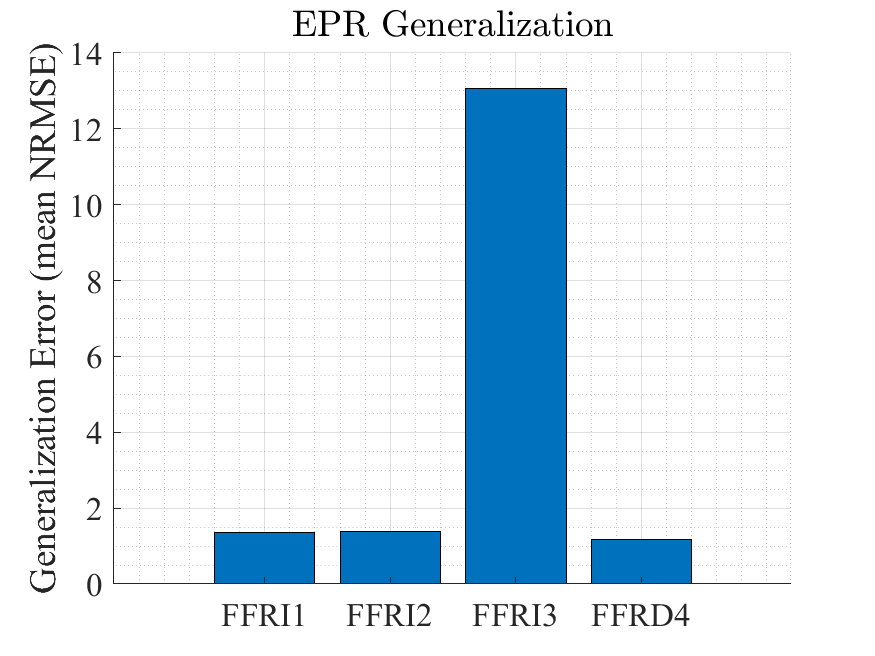
\includegraphics[width=\textwidth]{EPRANNGenE.png}
        \caption{}
        \label{fig:ANNGenEPR}
    \end{subfigure}
    \begin{subfigure}[b]{0.49\textwidth}
        \centering
        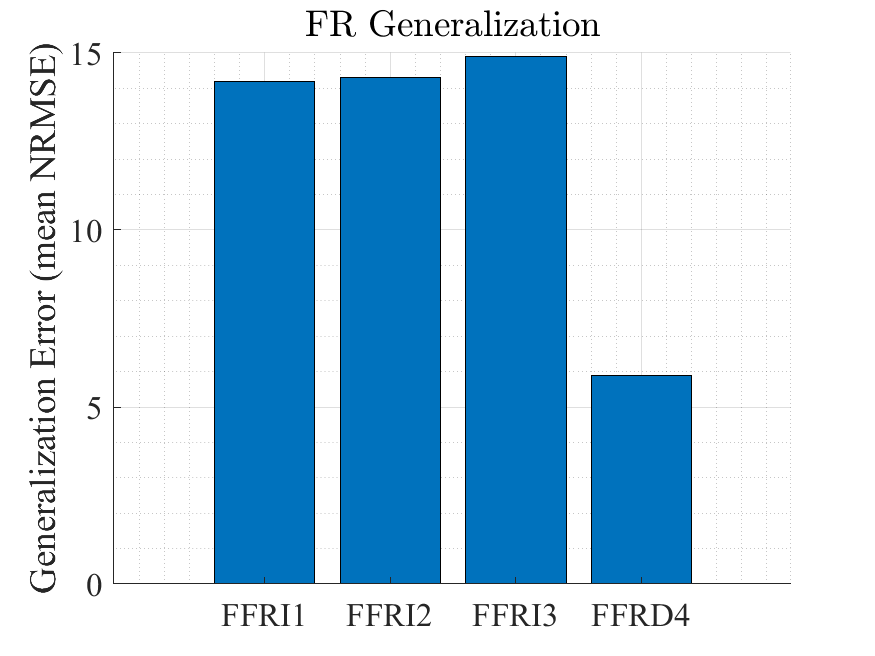
\includegraphics[width=\textwidth]{FRANNGenE.png}
        \caption{}
        \label{fig:ANNGenFR}
    \end{subfigure}
    \begin{subfigure}[b]{0.49\textwidth}
        \centering
        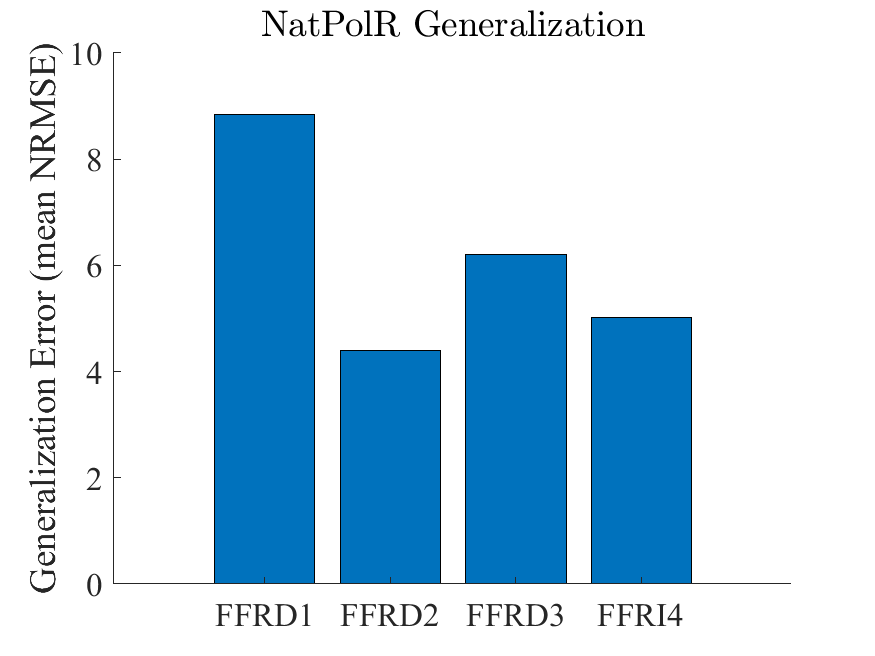
\includegraphics[width=\textwidth]{NatPolRANNGenE.png}
        \caption{}
        \label{fig:ANNGenNR}
    \end{subfigure}
    \begin{subfigure}[b]{0.49\textwidth}
        \centering
        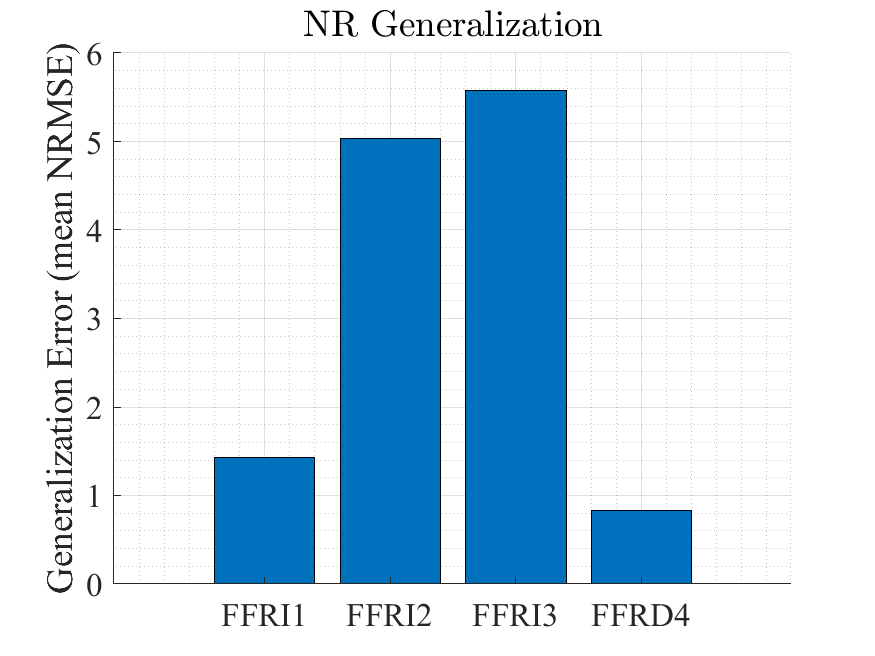
\includegraphics[width=\textwidth]{NRANNGenE.png}
        \caption{}
        \label{fig:ANNGenNatPolR}
    \end{subfigure}
    \begin{subfigure}[b]{0.49\textwidth}
        \centering
        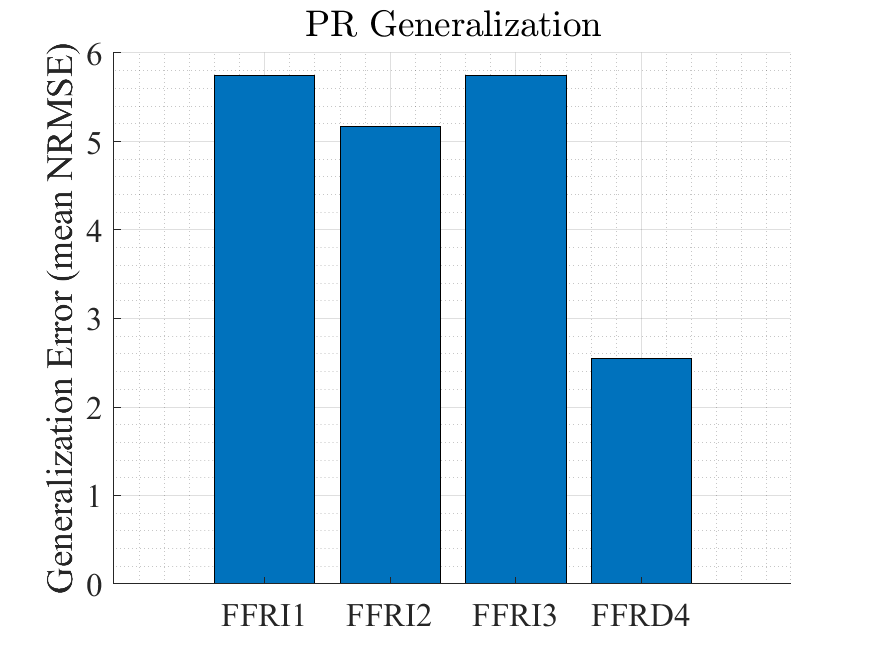
\includegraphics[width=\textwidth]{PRANNGenE.png}
        \caption{}
        \label{fig:ANNGenPR}
    \end{subfigure}
    \begin{subfigure}[b]{0.49\textwidth}
        \centering
        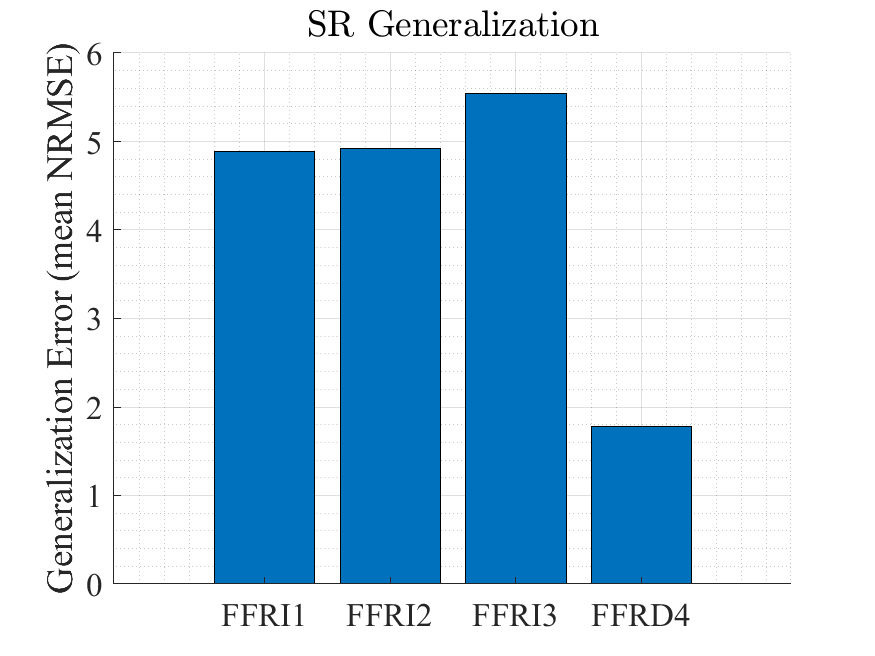
\includegraphics[width=\textwidth]{SRANNGenE.png}
        \caption{}
        \label{fig:ANNGenSR}
    \end{subfigure}
    \caption{Generalization error, based on a 10-fold cross-validation, for the (a) EPR, (b) FR, (c) NatPolR, (d) NR, (e) PR, and (f) SR materials. The best input combination is the one with the smallest generalization error, i.e. ff4.}
    \label{fig:ANNGen4}
\end{figure}

\begin{figure}[htbp!]
    \centering
    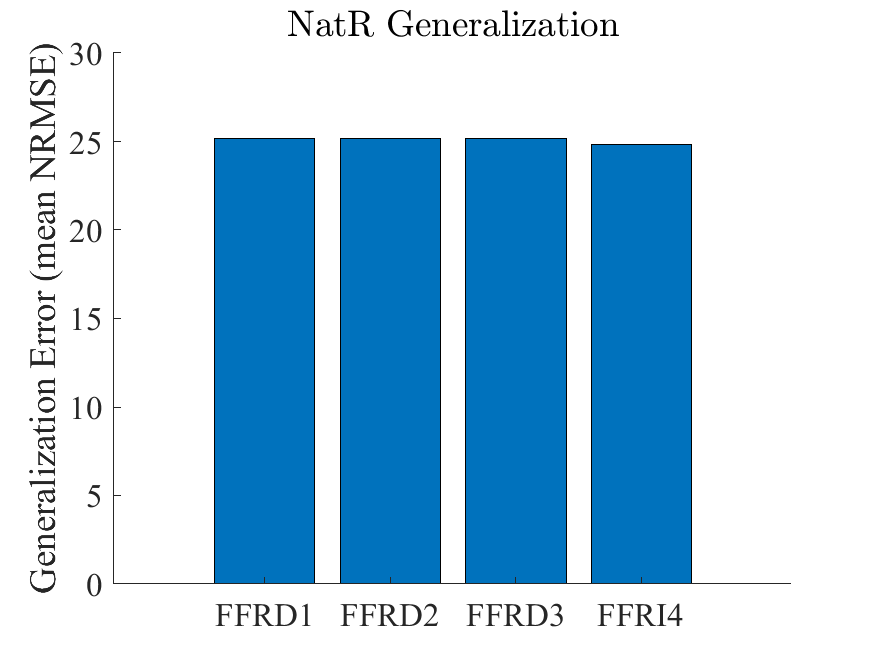
\includegraphics[width=0.49\textwidth]{NatRANNGenE.png}
    \caption{Generalization error, based on a 10-fold cross-validation, for the NatR material. The best input combination is the one with the smallest generalization error, i.e. ff4.}
    \label{fig:ANNGenNatR}
\end{figure}

In \Cref{fig:ANNGen4,fig:ANNGenNatR}, the ff4 architecture is identified as the one with the best generalization capabilities, i.e. smallest generalization error. This is the case for all the materials with the exception of the NatPolR material, for which the smallest generalization error was achieved by the ff2 architecture. Nonetheless, the difference between the ff4 and the ff2 architecture are minimal. Hence, following optimizations are based on the ff4 architecture. 
In \Cref{fig:ANNGen4,fig:ANNGenNatR}, it can also be appreciated the beneficial impact of increasing the length of the strain history provided to the ANN. Nonetheless, these benefits are less than when using the strain rate as input. Initially, a couple of architecture were proposed, which contained the past values of the stress response of the material. The achieved generalization error on these architectures was at least one order of magnitude lower than the errors reported in \Cref{fig:ANNGen4,fig:ANNGenNatR}. The latter is misleading in thinking that architectures which have the past values of the stress as input are the best solution, because in a real application, this would translate into measuring the stress response of the material. This contradict the main reason behind developing a modelling tool to predict the mechanical response of soft materials being implemented in a series-viscoelastic actuator, which is: transforming the force control problem into a position control problem. In other words, in a real robotic application, the deformation of the soft material is measured and this information is used to estimate the force response of the material, ultimately relating this force with the force exerting by the actuator. Therefore, an ANN with such an architecture was discarded. Finally, the optimization performed in here showed that the best architecture for accounting the velocity-dependency of the stress-train curve of soft materials, is a Rate-Dependent one, specifically, the architecture code-named as ff4. The next optimization is focused on the number of neurons in the hidden layer.

\subsection{Analysis: Optimal number of neurons}

In the literature, the recommendation of having two to three neurons for each input of the ANN is mentioned. This recommendation seems to be in accordance to the number of neurons used in the documented implementations \cite{rodriguez2019application,kopal2018prediction,jenik2017sequential}. Nonetheless this is not true for all implementations \cite{yousef2011prediction,kopal2017modeling}. Moreover, the number of neurons must be kept at its minimum to avoid the ANN to over-fit the training dataset. Therefore, it is desirable to search for the optimal number of neurons which allow the developed ANN to achieve a desired accuracy. In here, the latter search is performed, initially, for a range of 1 to 10 neurons. Although, this range was further expanded to up to 20 neurons because the desired performance was not met for most of the materials. The coefficient of determination, $R^2$ value, is used to assess the performance of the ANNs, in combination with the multiple training session of randomized datasets method. An adequate performance is such with a value of $R^2>0.995$. Moreover, the multiple training method performed consist of training each developed ANN, in the range from 1 to 20 neurons, five times. In each session, the whole dataset is randomized and divided into training and test subsets. The main objective of this optimization process limit the resources of the developed ANN, i.e. to avoid over-fitting, by finding the training session with the minimum number of neurons that has a value of $R^2>0.99$. A similar process to this, but using the percentage of correct prediction, is documented in \cite{zhang2002dynamic}

In this optimization, the complete dataset available for each material is subdivided to allocate 80\% of the data for training and 20\% for testing. As previously mentioned, no validation subset is required when using the Bayesian Regularization algorithm. Moreover, the list of hyper-parameters used in this case are compiled in \Cref{tbl:ANN_nueronOpt}.

\begin{table}[htbp!]
    \centering
    \caption{Proposed hyper-parameters for the number of neurons optimization}
    \begin{tabular}{l m{1cm} l}
    \toprule
    \multicolumn{3}{l}{Fixed Hyper-parameters} \\
    \hline
    Architecture               & & ff4 (see \Cref{tbl:ANNArchitectures})\\
    Number of Neurons           & & 1 to 20 \\
    Data Set Size               & & 100\% of available data\\
    Data Division               & & 80\% for training, 20\% for testing\\
    Error Measure               & & $R^2$ value\\
    Validation Method           & & Multiple Training with Random Test Sets\\
    \bottomrule
    \end{tabular}
    \label{tbl:ANN_nueronOpt}
\end{table}

The results of this optimization are illustrated in \Cref{fig:TrialsNeurons1,fig:TrialsNeurons2,fig:TrialsNeurons3}. In there, the achieved generalization errors, based on the mean NRMSE value from the executed tests, and the $R^2$ values, are presented. Regarding the generalization error, the benefits of having more than ten neurons are negligible, and even detrimental in some cases. This is observed in \Cref{fig:GenNeuronsNatR,fig:GenNeuronsNatPolR,fig:GenNeuronsPR}.

The $R^2$ value, or coefficient of determination, indicates the fraction of the data variation which is explained by the ANN model. Traditionally, a $R^2$ value closer to 1 indicates a very good model fit. However, in the field of ANNs, a very high $R^2$ value could actually indicate over-fit in the developed ANN. In general, most of the achieved $R^2$ values are below the desired threshold of $R^2>0.99$. Only the ANN models for the EPR and NR materials are able to meet the latter threshold. Furthermore, the lowest $R^2$ value is reported for the NatR material. The PL-SLS model also performed poorly for this specific material. Nonetheless, the information presented in \Cref{fig:TrialsNeurons1,fig:TrialsNeurons2,fig:TrialsNeurons3} is useful for the selection of the most optimal number of neurons.

\begin{figure}[htbp!]
	\centering
    \begin{subfigure}[b]{0.49\textwidth}
        \centering
        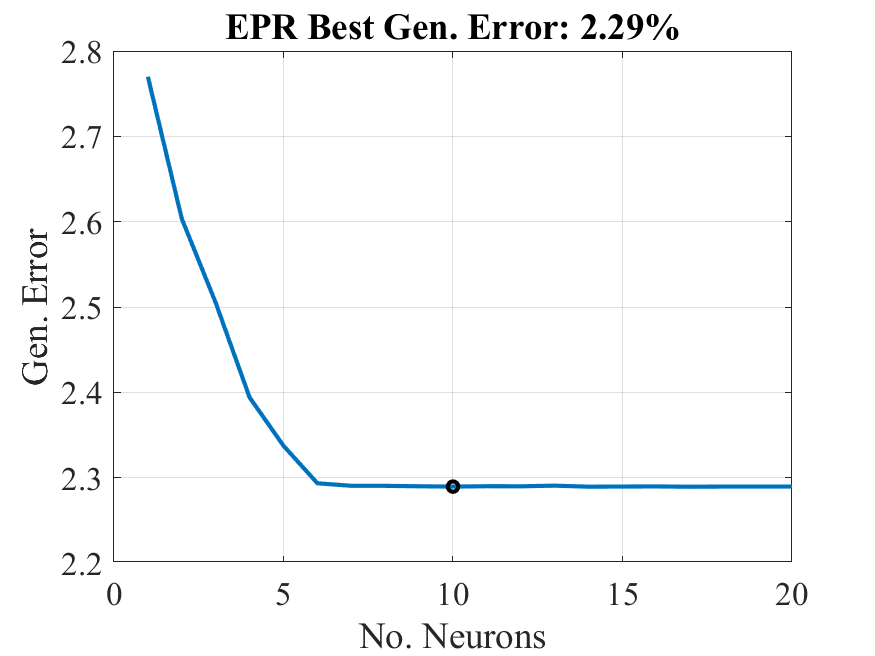
\includegraphics[width=\textwidth]{EPRGeNeurons.png}
        \caption{}
        \label{fig:GenNeuronsEPR}
    \end{subfigure}
    \begin{subfigure}[b]{0.49\textwidth}
        \centering
        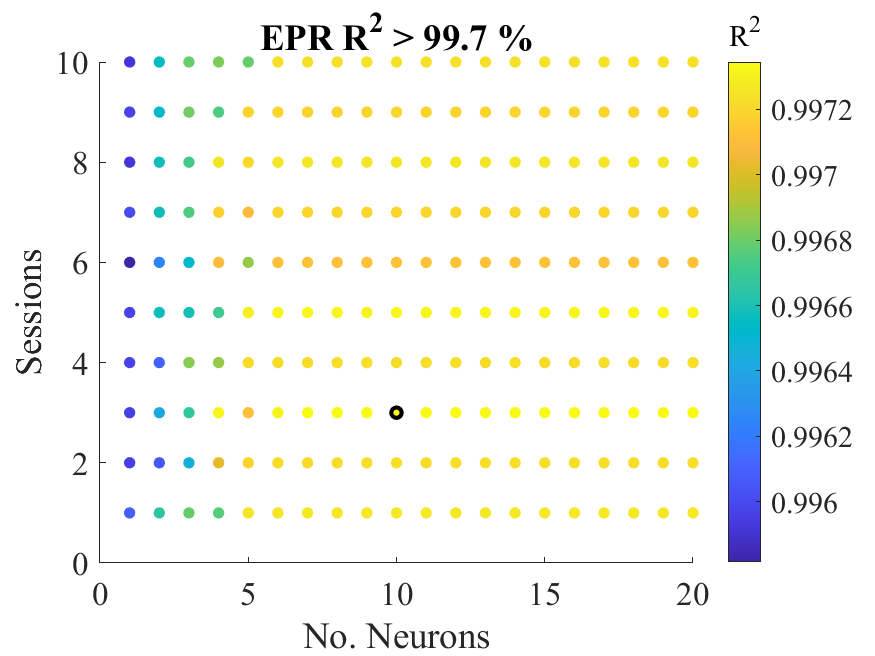
\includegraphics[width=\textwidth]{EPRR2TrialsNeurons.png}
        \caption{}
        \label{fig:TrialsNeuronsEPR}
    \end{subfigure}
    \begin{subfigure}[b]{0.49\textwidth}
        \centering
        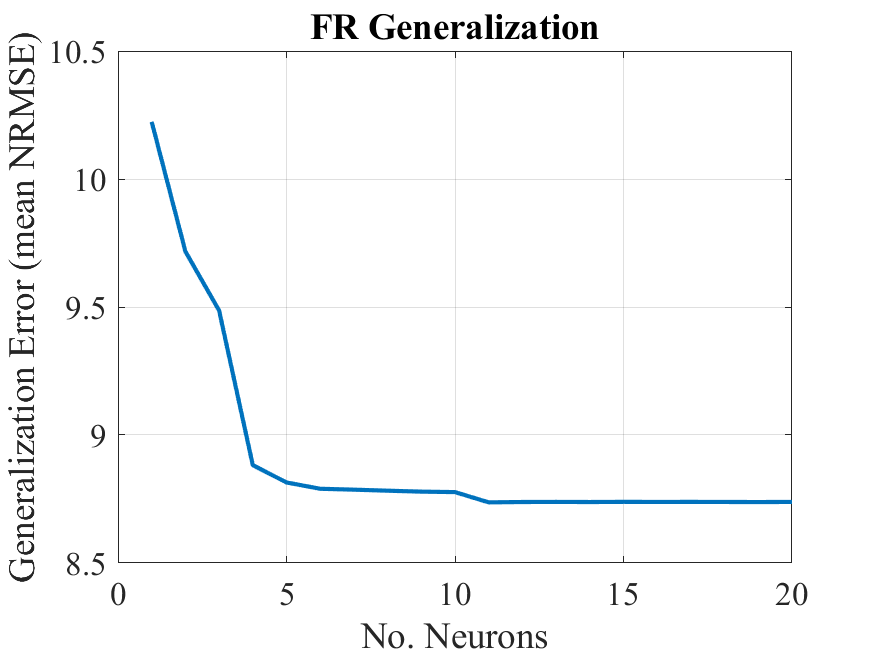
\includegraphics[width=\textwidth]{FRGeNeurons.png}
        \caption{}
        \label{fig:GenNeuronsFR}
    \end{subfigure}
    \begin{subfigure}[b]{0.49\textwidth}
        \centering
        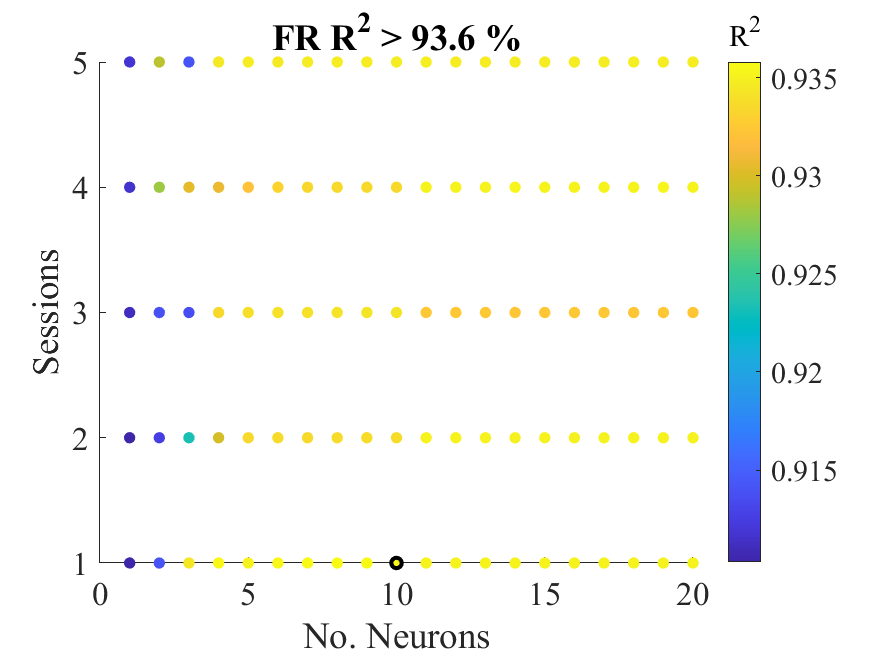
\includegraphics[width=\textwidth]{FRR2TrialsNeurons.png}
        \caption{}
        \label{fig:TrialsNeuronsFR}
    \end{subfigure}
    \begin{subfigure}[b]{0.49\textwidth}
        \centering
        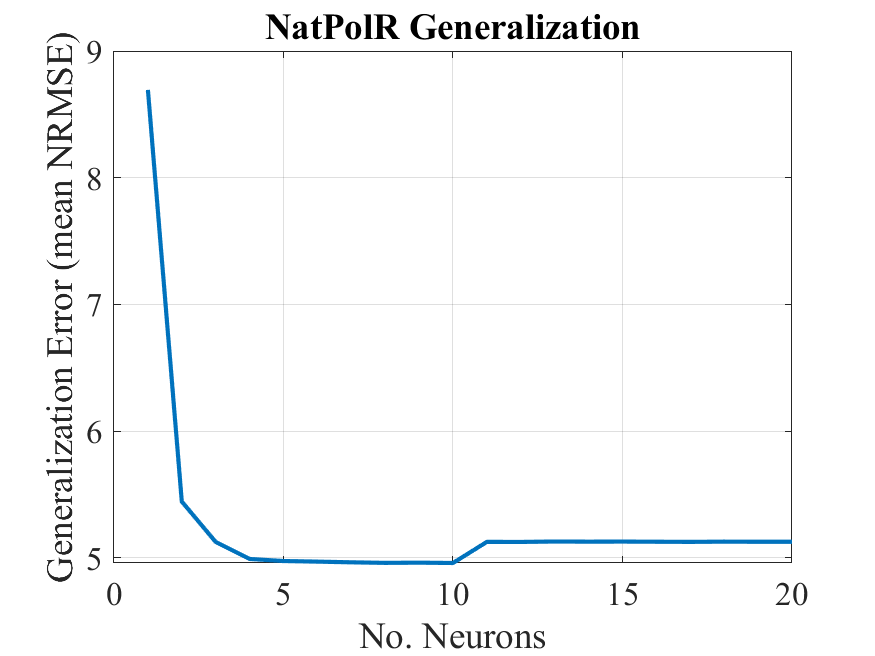
\includegraphics[width=\textwidth]{NatPolRGeNeurons.png}
        \caption{}
        \label{fig:GenNeuronsNatPolR}
    \end{subfigure}
    \begin{subfigure}[b]{0.49\textwidth}
        \centering
        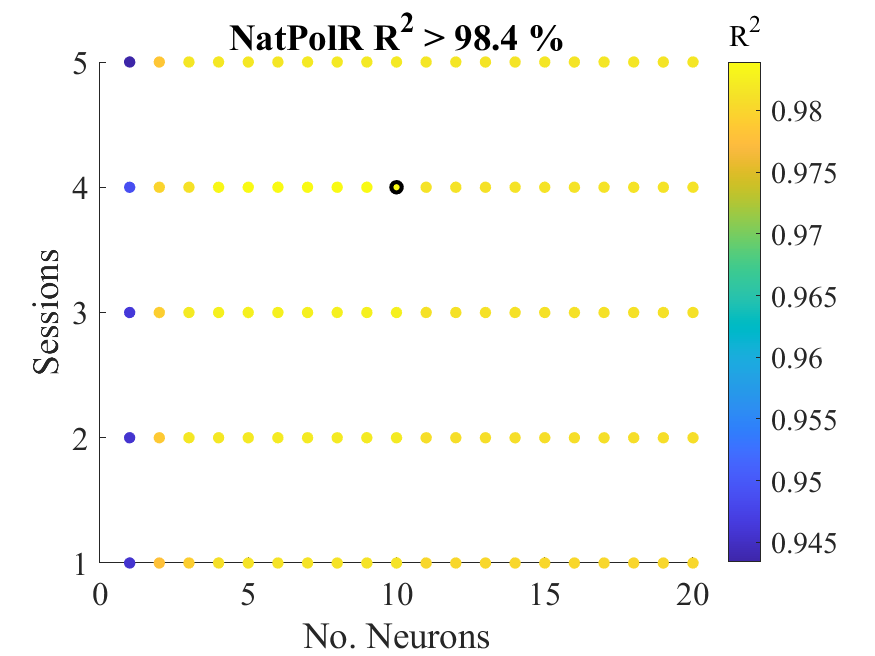
\includegraphics[width=\textwidth]{NatPolRR2TrialsNeurons.png}
        \caption{}
        \label{fig:TrialsNeuronsNatPolR}
    \end{subfigure}
    \caption{Impact of the number of neurons on the Generalization error (a), (c), (e), and the $R^2$ value (b), (d), (f), for the EPR, FR, and NatPolR materials. A total of five training session were executed per number of neurons. The best $R^2$ value is circled.}
    \label{fig:TrialsNeurons1}
\end{figure}

\begin{figure}[htbp!]
	\centering
    \begin{subfigure}[b]{0.49\textwidth}
        \centering
        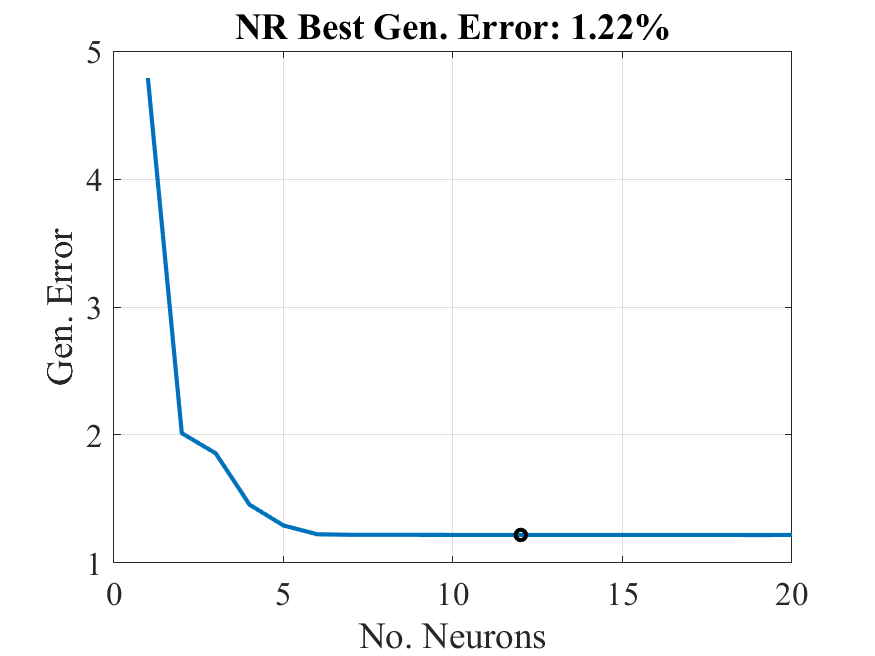
\includegraphics[width=\textwidth]{NRGeNeurons.png}
        \caption{}
        \label{fig:GenNeuronsNR}
    \end{subfigure}
    \begin{subfigure}[b]{0.49\textwidth}
        \centering
        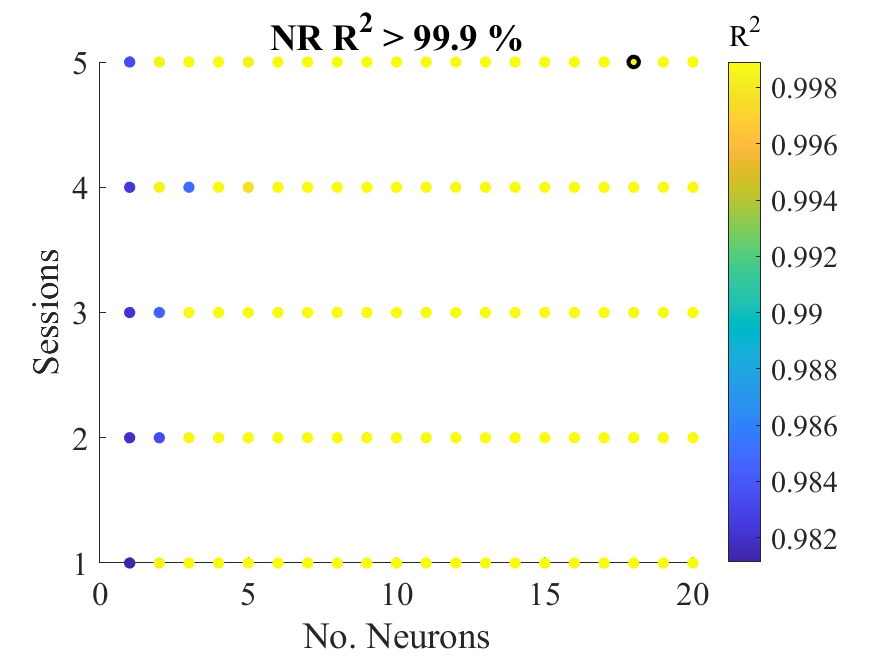
\includegraphics[width=\textwidth]{NRR2TrialsNeurons.png}
        \caption{}
        \label{fig:TrialsNeuronsNR}
    \end{subfigure}
    \begin{subfigure}[b]{0.49\textwidth}
        \centering
        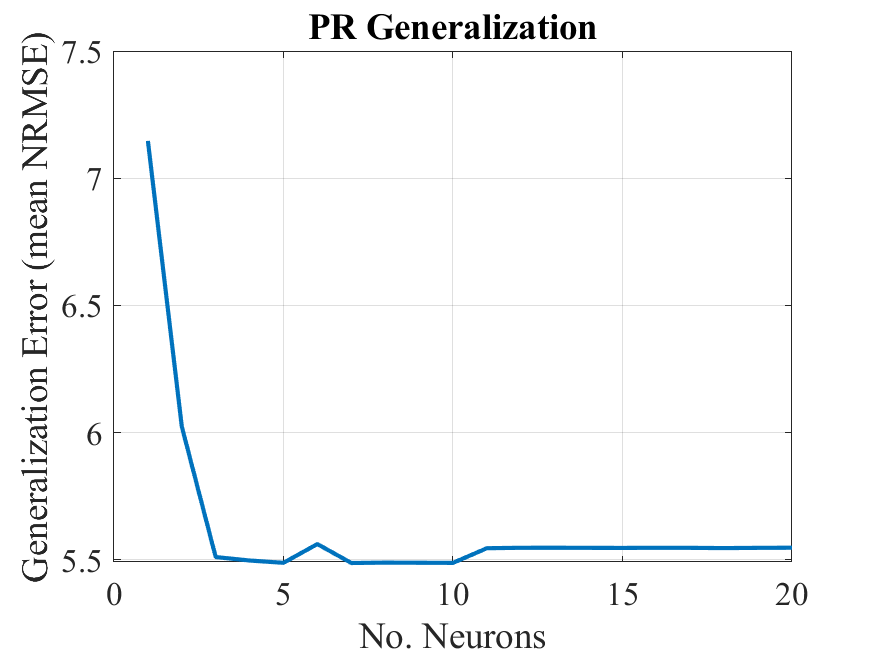
\includegraphics[width=\textwidth]{PRGeNeurons.png}
        \caption{}
        \label{fig:GenNeuronsPR}
    \end{subfigure}
    \begin{subfigure}[b]{0.49\textwidth}
        \centering
        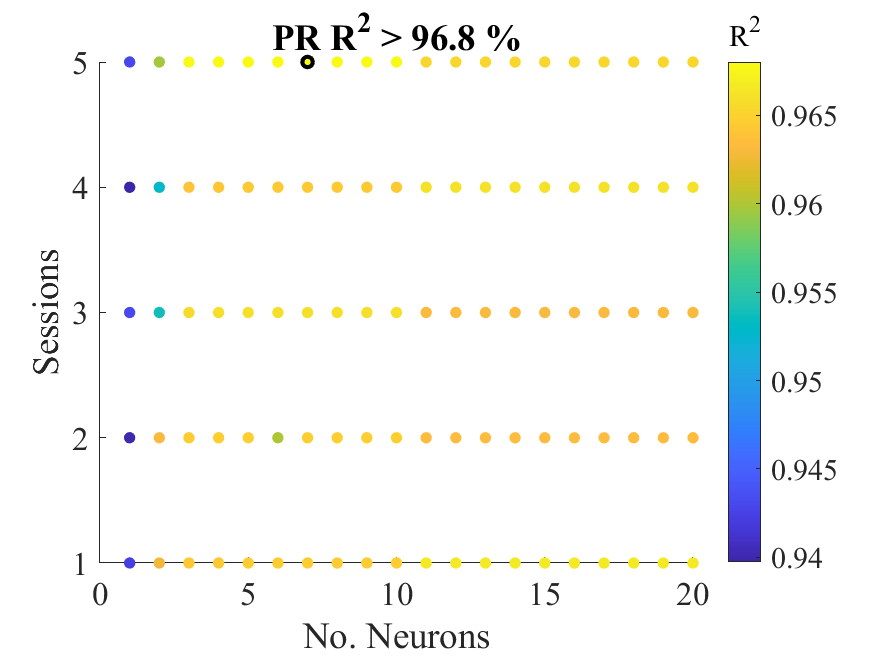
\includegraphics[width=\textwidth]{PRR2TrialsNeurons.png}
        \caption{}
        \label{fig:TrialsNeuronsPR}
    \end{subfigure}
    \begin{subfigure}[b]{0.49\textwidth}
        \centering
        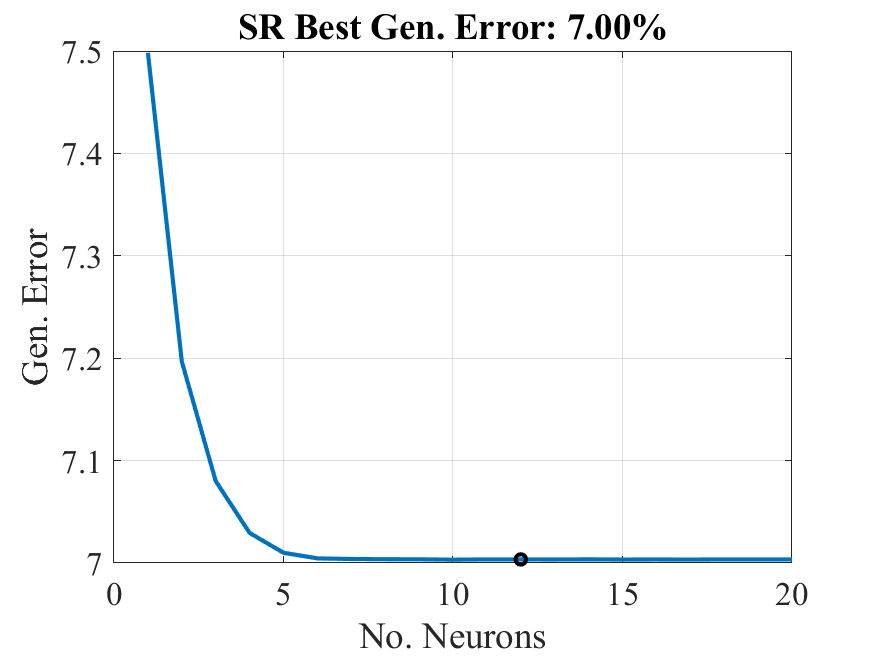
\includegraphics[width=\textwidth]{SRGeNeurons.png}
        \caption{}
        \label{fig:GenNeuronsSR}
    \end{subfigure}
    \begin{subfigure}[b]{0.49\textwidth}
        \centering
        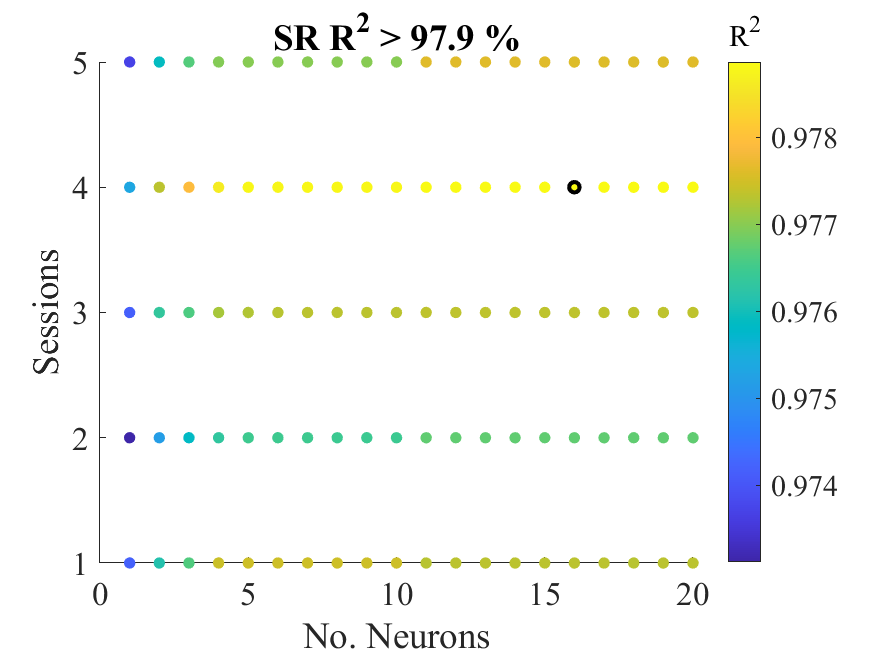
\includegraphics[width=\textwidth]{SRR2TrialsNeurons.png}
        \caption{}
        \label{fig:TrialsNeuronsSR}
    \end{subfigure}
    \caption{Impact of the number of neurons on the Generalization error (a), (c), (e), and the $R^2$ value (b), (d), (f), for the NR, PR, and SR materials. A total of five training session were executed per number of neurons. The best $R^2$ value is circled.}
    \label{fig:TrialsNeurons2}
\end{figure}

\begin{figure}[htbp!]
	\centering
    \begin{subfigure}[b]{0.49\textwidth}
        \centering
        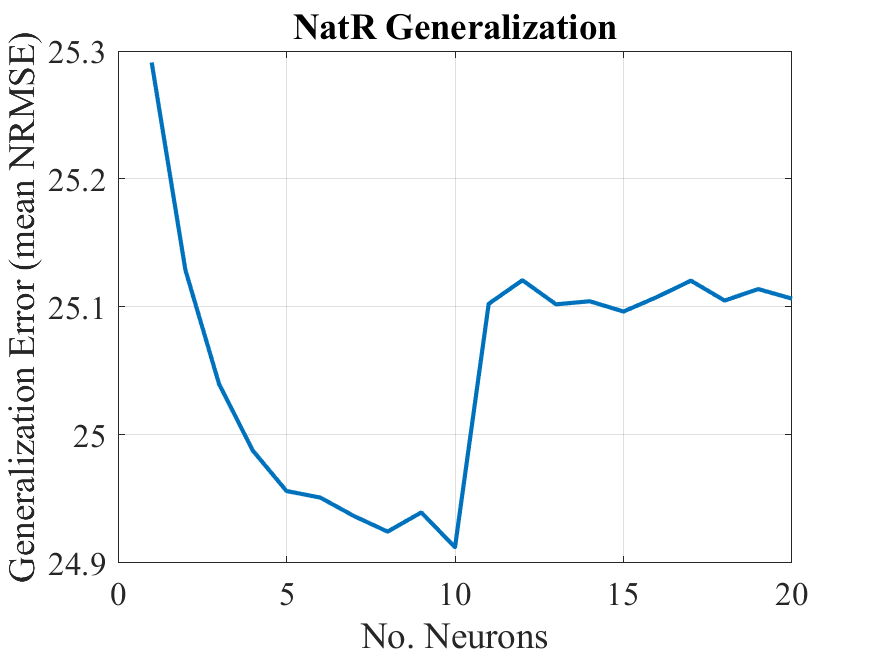
\includegraphics[width=\textwidth]{NatRGeNeurons.png}
        \caption{}
        \label{fig:GenNeuronsNatR}
    \end{subfigure}
    \begin{subfigure}[b]{0.49\textwidth}
        \centering
        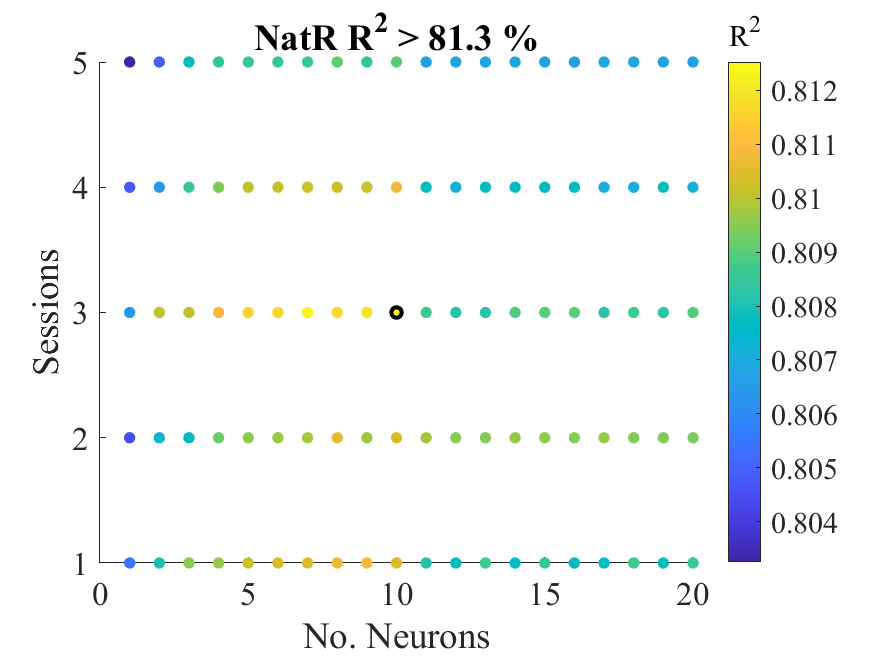
\includegraphics[width=\textwidth]{NatRR2TrialsNeurons.png}
        \caption{}
        \label{fig:TrialsNeuronsNatR}
    \end{subfigure}
    \caption{Impact of the number of neurons on the Generalization error (a) and the $R^2$ value (b), for the NatR material. A total of five training session were executed per number of neurons. The best $R^2$ value is circled.}
    \label{fig:TrialsNeurons3}
\end{figure}

The ANN with the optimal number of neurons must have the right combination of good accuracy (small NRMSE), low number of neurons, and high $R^2$ values. The first parameter to consider is the $R^2$ value. For the cases in which the threshold of this value is achieved, i.e. $R^2 > 0.99$, the optimal candidate is such in which the latter threshold is met with the minimum NRMSE and the minimum number of neurons. For the cases in which the threshold is not achieved, a closer look is given to the NRMSE to detect if an increase in the number of neurons translate in an improvement of the NRMSE. Following these conditions, the optimal number of neurons per soft material are extracted and presented in \Cref{tbl:ANNvsSLS}. In here, the PL-SLS model is also compared against the developed ANN model.

\begin{table}[htbp!]
    \centering
    \caption{Best ANN candidate compared against the PL-SLS model. The generalization error is based on the mean NRMSE value. In the case of the PL-SLS the latter is based on the mean NRMSE value from the available strain rates in \Cref{fig:GenAlmostAll,fig:GenOtherAll}}
    \begin{tabular}{p{1em} l ccccccc}
    \toprule
                    &                   & EPR   & FR    & NatPolR & NR  & PR    & SR    & NatR\\
    \hline
    \multicolumn{9}{l}{ANN model}\\
    &Generalization Error (\%)          & 2.3   & 8.8   & 4.9   & 1.2   &5.5    & 7     &   24.9\\
    &No. of Neurons                     & 6     & 10    & 10    & 6     &7      & 6     &   10\\
    &$R^2$ @ No. of Neurons             & 99.7  & 93.4  & 98.2  & 99.8  &96.5   & 97.7  &   81\\
    \midrule
    \multicolumn{9}{l}{PL-SLS model}\\
    &Generalization Error (\%)          & 21    & 34.2  & 8.4   & 20.8  & 31.6  & 3.2   & 258\\
    &Tolerance Criteria                 & 40    & 90    & 20    & 50    & 10    & 90    & 50\\
    &Strain Segments                    & 12    & 8     & 9     & 12    & 12    & 3     & 8\\
    \bottomrule
    \end{tabular}
    \label{tbl:ANNvsSLS}
\end{table}

From \Cref{tbl:ANNvsSLS} it can be observed that the ANN model have much better generalization capabilities in comparison to the PL-SLS model. However, the generalization error from both models is calculated slightly different. In the ANN model, the generalization error is the mean NRMSE value from all the trainins sessions performed. Wheres, in the PL-SLS, the generalization error is the mean NRMSE value among the other predicted strain rates, as illustrated in \Cref{fig:GenAlmostAll,fig:GenOtherAll}. Nonetheless, the generalization error is very useful to indicate the performance of both models when accounting for the velocity-dependancy of the stress response, i.e. different strain rates.

Interestingly enough, the PL-SLS model actually performs better than the ANN for the SR material. This is the only soft material, in which the tensile strength tests had to be performed using the 250 mm/min strain rates, instead of the recommended 500 mm/min. The latter was identified to have aide the PL-SLS model in achieved the same NRMSE for both the strain rates of 250 mm/min and 250 mm/min available for this material. Adding to this, the PL-SLS model was found to perform better for the soft materials which exhibited a more dominant elastic behaviour than a viscous behaviour. Therefore, it can be concluded that the stress response of the SR material is free of any velocity-dependency, which ultimately allowed the PL-SLS model to achieve good accuracy. 

The combination of inputs used for the developed ANN, of strain and strain rate, could be playing a role in the slightly worse performance of the ANN model in comparison to the PL-SLS model. In other worse, it could be possible that the ANN is not able to find a relationship between the strain rate and the stress response of the material, and hence that input is proven detrimental to the achieved accuracy rather than improving it.

Nonetheless, the developed ANN models have proven to be adequate for modeling the velocity-dependency of the stress response of viscoelastic materials, due to the small NRMSE achieved. The next step is to validate the performance of both models in a real robotic application, which is describes in the following chapter.

\section{Summary}

%this work \cite{xu2019artificial} an ANN which accounts for the strain rate of the materials is trained with three different strain rates. The trained and validated ANN was used to predict the elastic modulus of the materials under unknown strain rates. 

In this chapter, a data-driven modeling approach is proposed and developed as an alternative to traditional model-driven approaches which can be very computational costly. Artificial neural networks has been successfully implemented is many applications, but the literature available of the prediction of the viscoelastic properties of soft materials is still scarce. 

In line with the literature, a feedforward artificial neural network is developed to model the viscoelastic properties of seven soft materials. The developed ANN model is aimed to be used in real robotics applications, specifically to predict the mechanical behaviour of the viscoelastic element found in a recent actuation technology, the series-viscoelastic actuator.

The process of developing the ANN model involved the optimization of the number of neurons in the hidden layer and the most appropriate selection of inputs and outputs, to account for the viscoelastic properties of the studies soft materials. The optimal number of neurons varied from one material to the other but it does not exceed 10 neurons. The inputs of the ANN were defined to be the strain and the strain rate of the materials. As the output, the ANN model was aimed to predict the stress response. in order to avoid over-fitting, the Bayesian Regularization algorithm was used instead of a traditional early stopping method based on the Levenberg-Marquardt algorithm.

The generalization capabilities of the ANN model was assessed using a multiple training approach in which the network was presented with slightly different data from a randomized test set. The mean normalized root mean square error from the latter training sessions is known as the generalization error. In general the ANN model performed better than the previously developed PL-SLS model in \Cref{sec:ChapterModellingLVM}. The only isolated case for which the PL-SLS model performs better than the ANN model is for the prediction of the SR material stress response. The latter could be attributed to the fact that the SR material stress response is not affected by the velocity, i.e. strain rate. Hence, having the strain rate as input to the ANN model could be detrimental to the performance of the network. Nonetheless, the question still remains on whether these different modeling approach could be implemented as part of a control system for the prediction, in real time, of the stress response of a viscoelastic material. This is investigated in the following chapter.